%
\section{Image filtering}
\label{sec:image-filtering}
Previously on subsection \ref{sec:face-detection} it was mentioned how to detect faces using computer vision. After that, it necessary to use filters and apply them in the user's face in order to have the Snapchat alike filters, for example like in Fig.~\ref{fig:snapchat-filter}.
%
\begin{figure}[!hbt]
\centering
    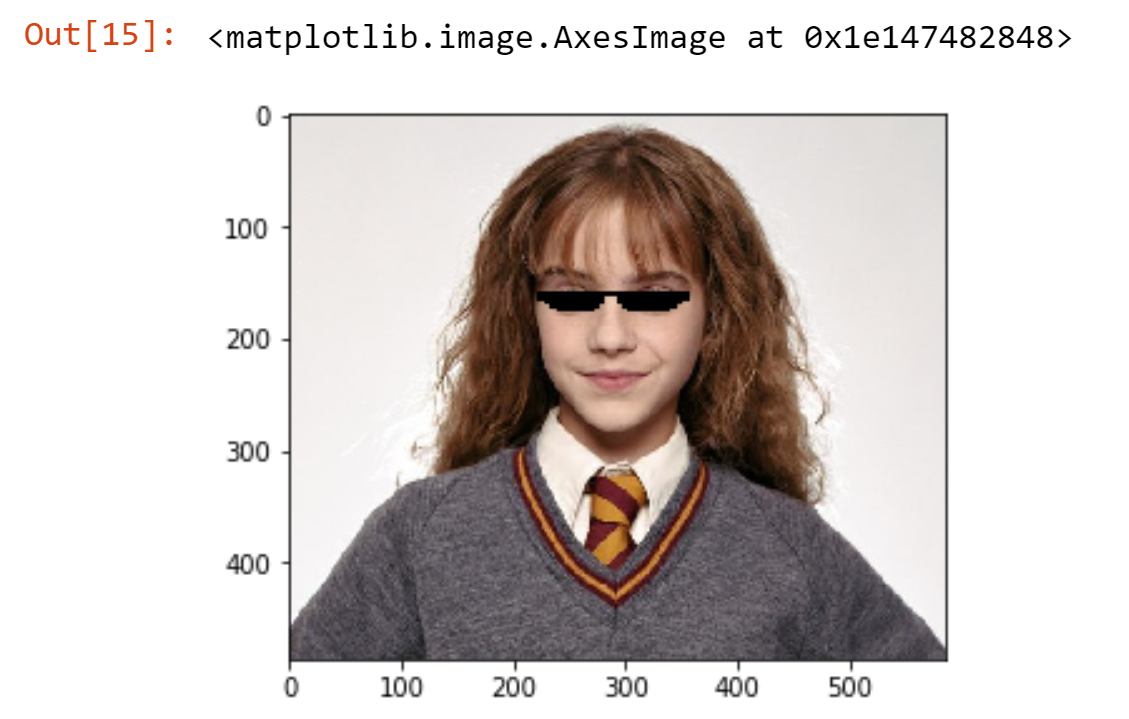
\includegraphics[width=0.8\textwidth]{./img/snapchat-filter.png}
  \caption{Example of Snapchat like filter(withdrawn from~\cite{snapchat-filter})}%
\label{fig:snapchat-filter}
\end{figure}

\subsection{Using filters with OpenCV}
\label{sec:filter-opencv}

Using \texttt{OpenCV} it is also possible to implement that kind of Snapchat like filters in a easy way.
In Listing \ref{lst:filter-ex} is an example on how to implement that type of filters using python.
Basically, it are detected all the faces in the image and it is made the scale of the image filters depending on the size of the face, this makes the filter look more real in the user's face.
The filter is only an overlayed image, in this case are three images, a mustache, a cigar and glasses. These three images are then scaled and putted on the specific point of the face too look like the user has a mustache, sunglasses and a cigar.
%
\lstinputlisting[language=python, firstline=1,
caption={Example on how to implement filters in faces},
label=lst:filter-ex,
style= custom-cpp]{./listing/filter-example.py}

Now, it is only necessary to translate this type of approach to C++ language, which is not that hard to do because there is already a knowledge on how to detect faces using this library. 
%%% Local Variables:
%%% mode: latex
%%% TeX-master: "../../../dissertation"
%%% End:
